\documentclass{beamer}
\usepackage{units,multicol,booktabs,tikz,xparse,tikz-3dplot,animate,mathtools}
\usetikzlibrary{arrows.meta,calc,shapes,angles,quotes,patterns}

\graphicspath{{Images/}}

%Display framenumber in footer
\newcommand*\oldmacro{}%
\let\oldmacro\insertshorttitle%
\renewcommand*\insertshorttitle{%
  \oldmacro\hfill%
  \insertframenumber\,/\,\inserttotalframenumber}

%Choose colors for themes
\definecolor{myblue}{rgb}{0.2,0.2,0.7} %Default Warsaw
\definecolor{myred}{RGB}{165,8,8}
\definecolor{myviolet}{RGB}{100,8,165}
\definecolor{mygreen}{RGB}{0,132,15}

%Tikz colors
\definecolor{bluegrid}{RGB}{197,207,224}

% Initialize default color theme
\setbeamercolor{author in head/foot}{bg=black} 		%1501 foot
\setbeamercolor{subsection in head/foot}{bg=myblue} 	% lecture title foot
\setbeamercolor{section in head/foot}{bg=black} 		% frametitle gradient
\setbeamercolor{frametitle}{bg=myblue} 				%frametitle primary color
\setbeamercolor{local structure}{fg=black}				%Necessary for enumerate
\setbeamercolor{item projected}{bg=myblue}			%itemize bullets

% iClicker environment color theme (to be used before \begin{frame} and after \end{frame})
\newenvironment{iclicker}
{
\setbeamercolor{author in head/foot}{bg=black} 		
\setbeamercolor{subsection in head/foot}{bg=myred} 	
\setbeamercolor{frametitle}{bg=myred}
\setbeamercolor{item projected}{bg=myblue}			
}{
\setbeamercolor{author in head/foot}{bg=black}
\setbeamercolor{subsection in head/foot}{bg=black} 
\setbeamercolor{frametitle}{bg=myblue}
\setbeamercolor{item projected}{bg=myblue}	
}
% Problem/example environment color theme
\newenvironment{myproblem}
{
\setbeamercolor{author in head/foot}{bg=black} 		
\setbeamercolor{subsection in head/foot}{bg=myviolet} 	
\setbeamercolor{frametitle}{bg=myviolet}
\setbeamercolor{item projected}{bg=myviolet}	 				
}{
\setbeamercolor{author in head/foot}{bg=black}
\setbeamercolor{subsection in head/foot}{bg=myblue} 
\setbeamercolor{frametitle}{bg=myblue}
\setbeamercolor{item projected}{bg=myblue}	
}

% iClicker enumerate box drawing
\newcommand{\tikzmark}[1]{\tikz[overlay,remember picture] \node (#1) {};}

% Macros
\newcommand{\vect}[1]{\mathbf{#1}}
\newcommand{\vecth}[1]{\hat{\mathbf{#1}}}
\def\flb#1\fle{\begin{flalign*}#1\end{flalign*}} % begin / end full left align

% More Stuff
\usefonttheme[onlymath]{serif}
\setbeamercovered{invisible}
\hfuzz=60pt %Surpresses hbox full warnings by extending to 50pt
\newdimen\hfuzz
\vbadness = 10000 %Similar to hbox warning supression

% Mode
\mode<presentation>{\usetheme{Warsaw}}


% Generate Credentials
\title[Cosmological Fluctuations]{Cosmological Fluctuations in Standard and Conformal Gravity}
\author[Matthew Phelps]{Matthew Phelps}
\institute{Doctoral Degree Final Examination
\and 
\includegraphics[width=0.8 in]{uconn-logo.png} }
\date{June 02, 2020}
%%%%%%%%%%%%%%%%%%%%%%%%%%%%%%%%%%%%%%%%%%%%%%%%%%%%%%%%%%%%%%
%%%%%%%%%%%%%%%%%%%%%%%%%%%%%%%%%%%%%%%%%%%%%%%%%%%%%%%%%%%%%%

\begin{document}
\beamertemplatenavigationsymbolsempty %Remove navigation icons
\setbeamertemplate{enumerate item}{(\Alph{enumi})} %Set default enumeration style

%%%%%%%%%%%%%%%%%%%%%%%%%%%%%%%%%%%%%%%%%%%%%%%%%%%%%%%%%%%%%%
%%%%%%%%%%%%%%%%%%%%%%%%%%%%%%%%%%%%%%%%%%%%%%%%%%%%%%%%%%%%%%

\begin{frame}
\setcounter{framenumber}{0}
	\titlepage
\end{frame}

%%%%%%%%%%%%%%%%%%%%%%%%%%%%%%%%%

\begin{frame}{Overview}
	\begin{itemize}
		\item Introduction and Formalism
		\begin{itemize}
			\item Cosmological Geometries
			\item Einstein Gravity
			\item Perturbation Theory
			\item Gauge Transformations
		\end{itemize}
		\item Conformal Gravity
	\end{itemize}
\end{frame}

%%%%%%%%%%%%%%%%%%%%%%%%%%%%%%%%%


%%%%%%%%%%%%%%%%%%%%%%%%%%%%%%%%%

\begin{frame}{Cosmological Geometries R.W.}
	Comoving Robertson Walker geometry:
	\begin{eqnarray*}
	ds^2 &=& -dt^2 + a(t)^2 \tilde g_{ij}dx^i dx^j
	\nonumber\\
	&=& -dt^2 + a(t)^2\bigg[\frac{dr^2}{1-kr^2} + r^2 d\theta^2 + r^2 \sin^2\theta d\phi^2\bigg]
	\end{eqnarray*}
	3-Space Curvature Tensors,
	\begin{eqnarray*}
	R_{ijkl} = k(\tilde g_{jk}\tilde g_{il} - \tilde g_{ik}\tilde g_{jl}), \qquad R_{ij} = -3k\tilde g_{ij}, \qquad R = -6k
	\end{eqnarray*}
	with $k \in \{-1,0,1\}$. Define the conformal time
	\begin{eqnarray*}
		\tau = \int \frac{dt}{a(t)},
	\end{eqnarray*}
	\only<1>{
	\begin{eqnarray*}
		ds^2 = a(\tau)^2\bigg[-d\tau^2 + \frac{dr^2}{1-kr^2} + r^2 d\theta^2 + r^2 \sin^2\theta d\phi^2\bigg]
	\end{eqnarray*}
	}
	\only<2>{
	set $k=0$,
	\begin{eqnarray*}
		ds^2 = a(\tau)^2\bigg[-d\tau^2 + dr^2 + r^2 d\theta^2 + r^2 \sin^2\theta d\phi^2\bigg]
	\end{eqnarray*}		
	}
\end{frame}

%%%%%%%%%%%%%%%%%%%%%%%%%%%%%%%%%

%%%%%%%%%%%%%%%%%%%%%%%%%%%%%%%%%

\begin{frame}{Cosmological Geometries R.W. $k=\pm 1$}
	$k=1$
	\begin{eqnarray*}
		ds^2 = -dt^2 + a(t)^2\bigg[\frac{dr^2}{1-r^2} + r^2 d\theta^2 + r^2 \sin^2\theta d\phi^2\bigg]
	\end{eqnarray*}

	$k=-1$
	\begin{eqnarray*}
		ds^2 = -dt^2 + a(t)^2\bigg[\frac{dr^2}{1+r^2} + r^2 d\theta^2 + r^2 \sin^2\theta d\phi^2\bigg]
	\end{eqnarray*}
\end{frame}

%%%%%%%%%%%%%%%%%%%%%%%%%%%%%%%%%

\begin{frame}{Effective Physics Theories}
\begin{columns}
	\column{0.5\linewidth}
		\begin{itemize}
			\item<1-> General Relativity
				\begin{itemize}
					\item<2-> Geometric theory of gravitation
					\item<3-> Relativity of time
					\item<4-> Black holes, cosmology, gps
				\end{itemize}
			\item<5-> Newtonian Mechanics
				\begin{itemize}
					\item<6-> Gravity as a force
					\item<7-> $v \ll c$
					\item<8-> Breaks down around $\unit[1]{\mu m}$
				\end{itemize}
			\item<9-> Quantum Theory
				\begin{itemize}
					\item<10-> Quantum Mechanics
					\item<11-> Quantum Field Theory
					\item<12-> Fundamental Particles
					\item<13-> Probabilistic flow of quantum states
					\item<14-> Discrete physics properties
				\end{itemize}
		\end{itemize}
	\column{0.5\linewidth}
		\resizebox{\linewidth}{!}{ 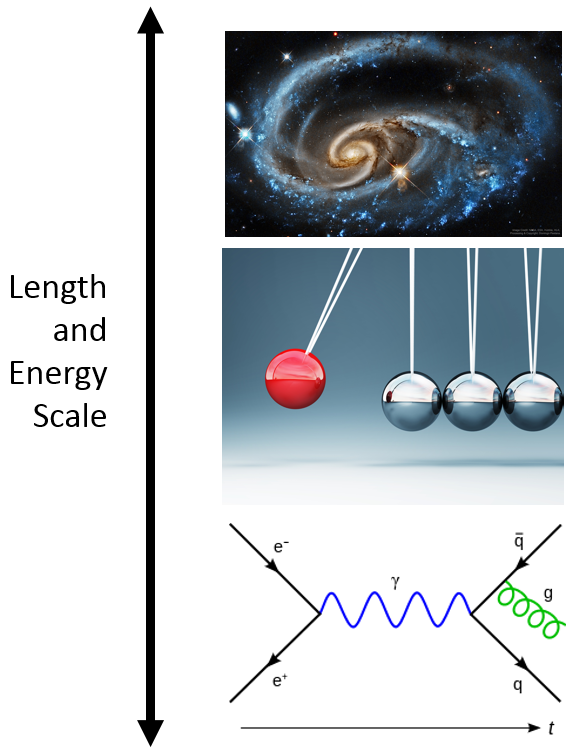
\includegraphics{scope.png} }
\end{columns}
\end{frame}

%%%%%%%%%%%%%%%%%%%%%%%%%%%%%%%%%

\begin{frame}{1D Kinematics}
	\begin{itemize}
		\item<1-> Independent of mass, force
		\item<2-> Restrict to $D=1$
		\item<3-> $\frac{d\vect F}{dt} = 0$
	\end{itemize}
\end{frame}

%%%%%%%%%%%%%%%%%%%%%%%%%%%%%%%%%
\begin{frame}{1D Motion: Analysis}
\begin{columns}
	\begin{column}{0.5\linewidth}
	\only<2>{
	 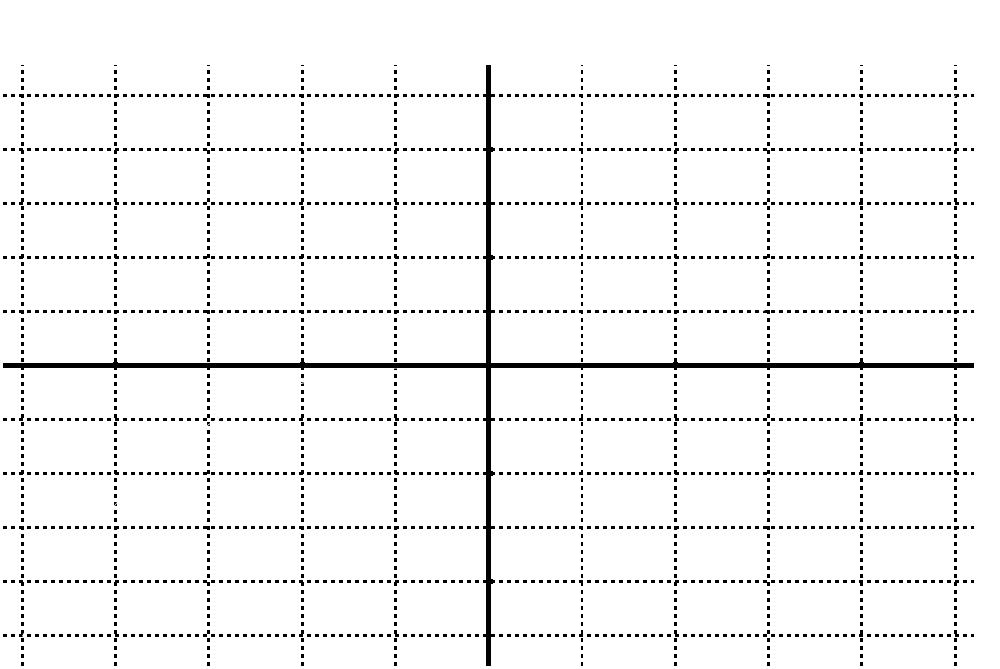
\includegraphics[width=\linewidth]{graph_1.jpg}
	}
	\only<3>{
	 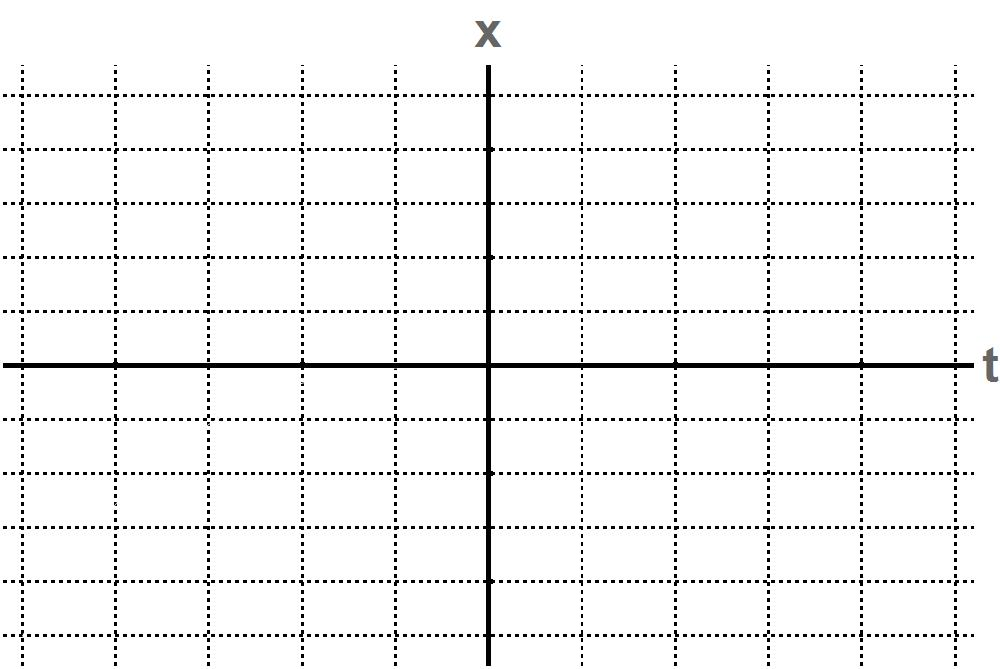
\includegraphics[width=\linewidth]{graph_2.jpg}
	}
	\only<4->{
	 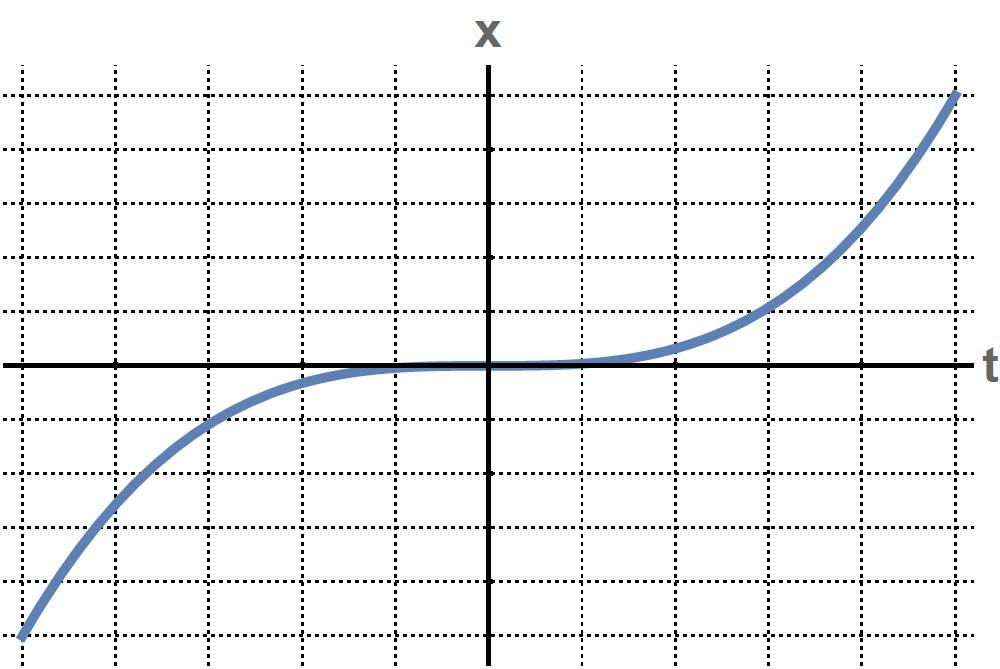
\includegraphics[width=\linewidth]{graph_3.jpg}
	}
	\begin{itemize}
	\item<5-> Distance
	\item <6-> Position (Displacement)
	\item <7-> Speed
	\item <8-> Velocity
	\end{itemize}
	\end{column}
	\begin{column}{0.5\linewidth}
		\resizebox{1\linewidth}{!}{
			\animategraphics[width=\linewidth,controls,loop]{30}{/1D_1/pic}{1}{201}
		}
	\end{column}
\end{columns}
\end{frame}

%%%%%%%%%%%%%%%%%%%%%%%%%%%%%%%%%
\begin{frame}{1D Motion: Average Velocity}
\begin{columns}
	\begin{column}{0.5\linewidth}
	 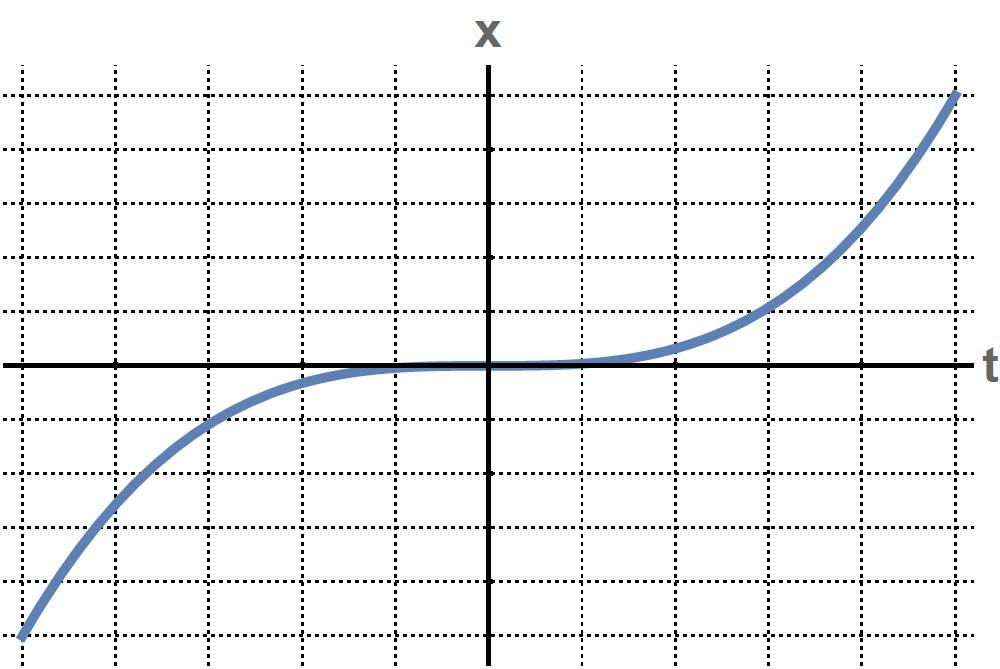
\includegraphics[width=\linewidth]{graph_3.jpg}
	\flb v_{avg}&= \frac{\Delta x}{\Delta t}\qquad |v|=\text{speed}&\fle
	\visible<2->{ What about $v(t)$? }
	\end{column}
	\begin{column}{0.5\linewidth}
		\resizebox{1\linewidth}{!}{
			\animategraphics[width=\linewidth,controls,loop]{30}{/1D_1/pic}{1}{201}
		}

	\end{column}
\end{columns}
\end{frame}

%%%%%%%%%%%%%%%%%%%%%%%%%%%%%%%%%
\begin{frame}{1D Motion: Instantaneous Velocity}
\begin{columns}
	\begin{column}{0.6\linewidth}
			\visible<1->{	\flb v_{avg}&= \frac{\Delta x}{\Delta t} = \frac{x(t_f)-x(t_i)}{t_f-t_i} &\fle }
			\vspace{-2mm}
			\visible<2->{ 	\flb t_f &= t_i + \Delta t &\fle
								\flb v_{avg}&= \frac{x(t_i +\Delta t)-x(t_i)}{\Delta t}& \fle
							}
			\visible<3->{ \flb v(t_i) &= \lim_{\Delta t\to 0} \frac{x(t_i + \Delta t)-x(t_i)}{\Delta t} =  \frac{dx}{dt} \bigg|_{t=t_i} &\fle
								\flb v &= \frac{dx}{dt} &\fle }
	\end{column}
	\begin{column}{0.4\linewidth}
		\resizebox{1\linewidth}{!}{
			\begin{tabular}{c}
				\hspace{-.1\linewidth}
				 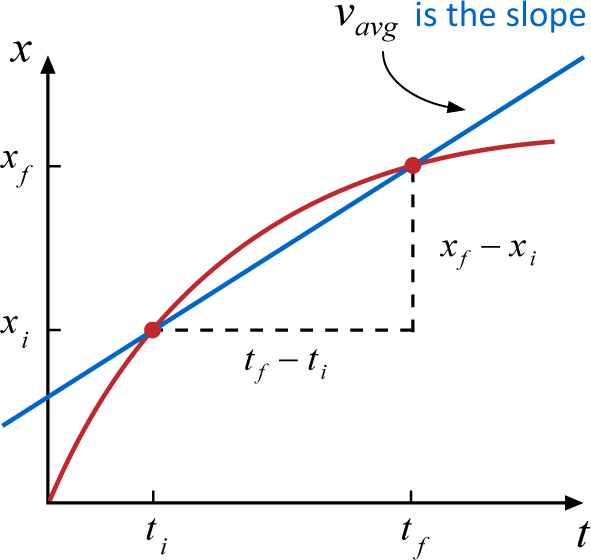
\includegraphics[width=\linewidth]{iv_1.jpg}\\
				\hspace{-.1\linewidth}
				 \visible<3->{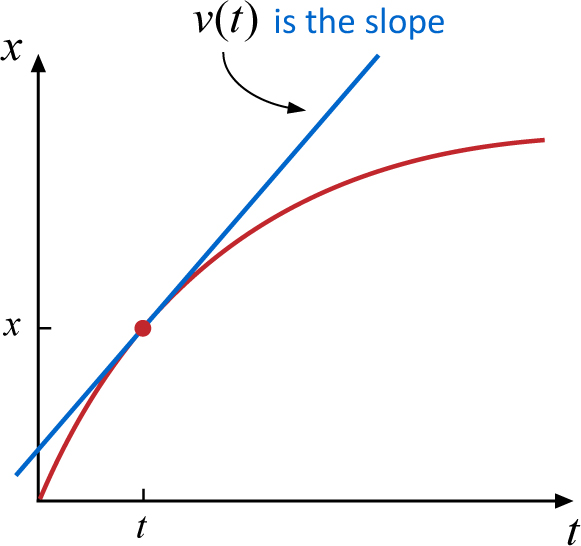
\includegraphics[width=\linewidth]{iv_2.jpg}}
			\end{tabular}
		}
	\end{column}
\end{columns}
\end{frame}

%%%%%%%%%%%%%%%%%%%%%%%%%%%%%%%%%
\begin{frame}{1D Motion: Average Acceleration}
\begin{columns}
	\begin{column}{0.6\linewidth}
		\flb a_{avg}&= \frac{\Delta v}{\Delta t}  = \frac{v(t_f)-v(t_i)}{t_f-t_i} &\fle
		What about $a(t)$? 
		\visible<2->{ 	\flb t_f &= t_i + \Delta t &\fle
							\flb a_{avg}&= \frac{v(t_i +\Delta t)-v(t_i)}{\Delta t}& \fle
		}
		\vspace{-2mm}
		\visible<3->{
							\flb a(t_i) &= \lim_{\Delta t\to 0} \frac{v(t_i + \Delta t)-v(t_i)}{\Delta t} =  \frac{dv}{dt} \bigg|_{t=t_i} &\fle
							\vspace{-2mm}
							\flb a &= \frac{dv}{dt} &\fle }
	\end{column}
	\begin{column}{0.4\linewidth}
		\hspace{-.3\linewidth}
		\resizebox{1.2\linewidth}{!}{
				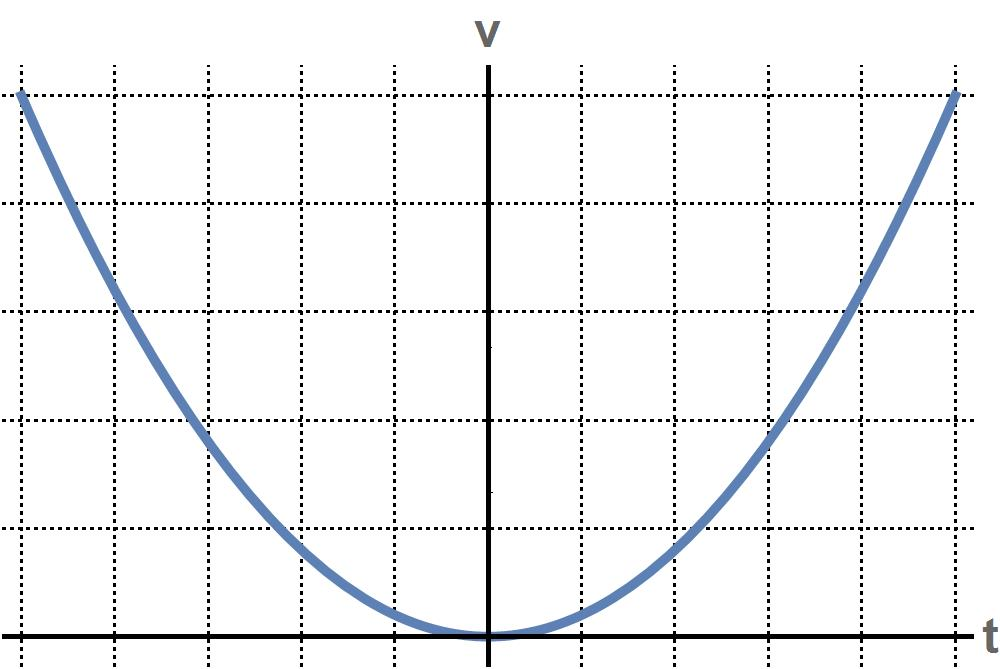
\includegraphics[width=\linewidth]{graph_4.jpg}
		}
		\vspace{20mm}
	\end{column}
\end{columns}
\end{frame}

%%%%%%%%%%%%%%%%%%%%%%%%%%%%%%%%%
\begin{frame}{1D Motion: Vocabulary}
\begin{columns}
	\begin{column}{0.5\linewidth}
	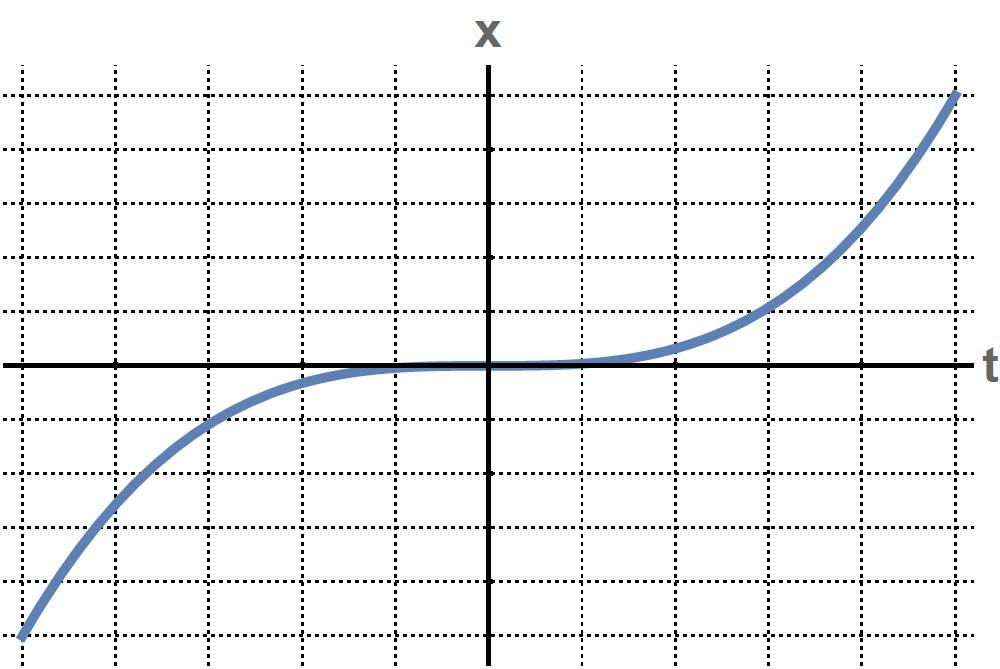
\includegraphics[width=\linewidth]{graph_3.jpg}
	\vspace{-4mm}
	\begin{itemize}
		\item  Distance
		\item  Displacement
		\item  Speed
		\item  Average Velocity
		\item  Instantaneous Velocity
		\item  Average Acceleration
		\item  Instantaneous Acceleration
	\end{itemize}
	\end{column}
	\begin{column}{0.5\linewidth}
		\resizebox{1\linewidth}{!}{
			\animategraphics[width=\linewidth,controls,loop]{30}{/1D_1/pic}{1}{201}
		}
	\end{column}
\end{columns}
\end{frame}

%%%%%%%%%%%%%%%%%%%%%%%%%%%%%%%%%
\begin{iclicker}
\begin{frame}{iClicker 1}
A particle's trajectory is given by the function 
\[ x(t) = (21+22t - 6t^2),\]
with $t,x$ in SI units. What is the average velocity from $t=1$ to $t=3$?
\begin{columns}
	\column{0.4\linewidth}
		\begin{enumerate}
			\item $\unit[2]{m/s}$
			\item $\unit[-4]{m/s}$
			\only<1>{\item $\unit[-2]{m/s}$}
			\only<2>{%
					\item \tikzmark{bl}$\unit[-2]{m/s}$\tikzmark{br}
					\tikz[overlay,remember picture]{\draw[red,thick]
	  				($(bl)+(-2.2em,1.0em)$) rectangle
	 				 ($(br)+(0.3em,-0.4em)$);}}
			\item $\unit[-8]{m/s}$
			\item $\unit[8]{m/s}$
		\end{enumerate}
	\column{0.6\linewidth}
	\visible<2->{
		\flb v_{avg}&= \frac{x(3)-x(1)}{3-1}&\\
			&= \frac{33-37}{2}&\\
			&= \unit[-2]{m/s}&
		\fle}
\end{columns}
\end{frame}
\end{iclicker}
%%%%%%%%%%%%%%%%%%%%%%%%%%%%%%%%%
\begin{iclicker}
\begin{frame}{iClicker 2}
What is the velocity (instantaneous) at $t=4$?
\\ \vspace{5mm}
\begin{columns}
	\column{0.2\linewidth}
		\begin{enumerate}
			\item $\unit[4]{m/s}$
			\only<1>{\item $\unit[0]{m/s}$}
			\only<2>{%
					\item \tikzmark{bl}$\unit[0]{m/s}$\tikzmark{br}
					\tikz[overlay,remember picture]{\draw[red,thick]
	  				($(bl)+(-2.2em,1.0em)$) rectangle
	 				 ($(br)+(0.3em,-0.4em)$);}}
			\item $\unit[1]{m/s}$
			\item Not enough information
		\end{enumerate}
	\column{0.8\linewidth}
	\resizebox{1\linewidth}{!}{
		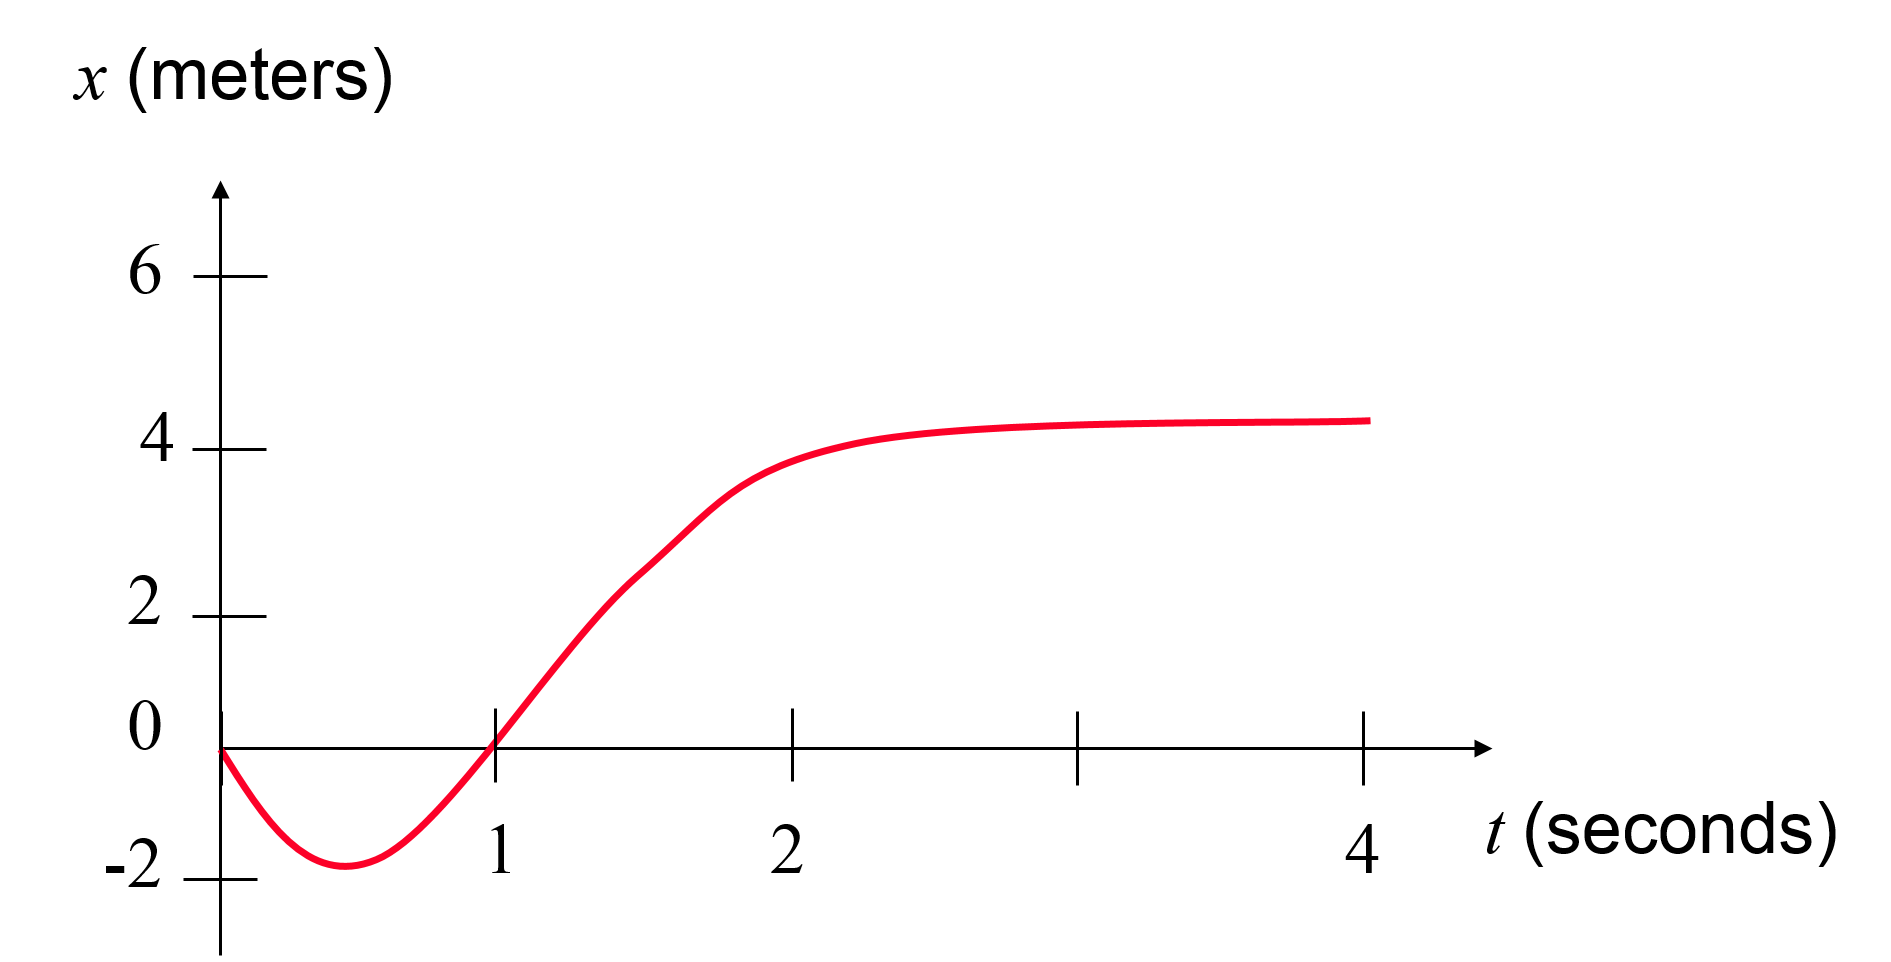
\includegraphics[width=\linewidth]{dfig1.png}
		}
\end{columns}
\end{frame}
\end{iclicker}

%%%%%%%%%%%%%%%%%%%%%%%%%%%%%%%%%
\begin{iclicker}
\begin{frame}{iClicker 3}
What is the average velocity over the first $4$ seconds?
\\ \vspace{5mm}
\begin{columns}
	\column{0.2\linewidth}
		\begin{enumerate}
			\item $\unit[-2]{m/s}$
			\item $\unit[4]{m/s}$
			\only<1>{\item $\unit[1]{m/s}$}
			\only<2>{%
					\item \tikzmark{bl}$\unit[1]{m/s}$\tikzmark{br}
					\tikz[overlay,remember picture]{\draw[red,thick]
	  				($(bl)+(-2.2em,1.0em)$) rectangle
	 				 ($(br)+(0.3em,-0.4em)$);}}
			\item Not enough information
		\end{enumerate}
	\column{0.8\linewidth}
	\resizebox{1\linewidth}{!}{
		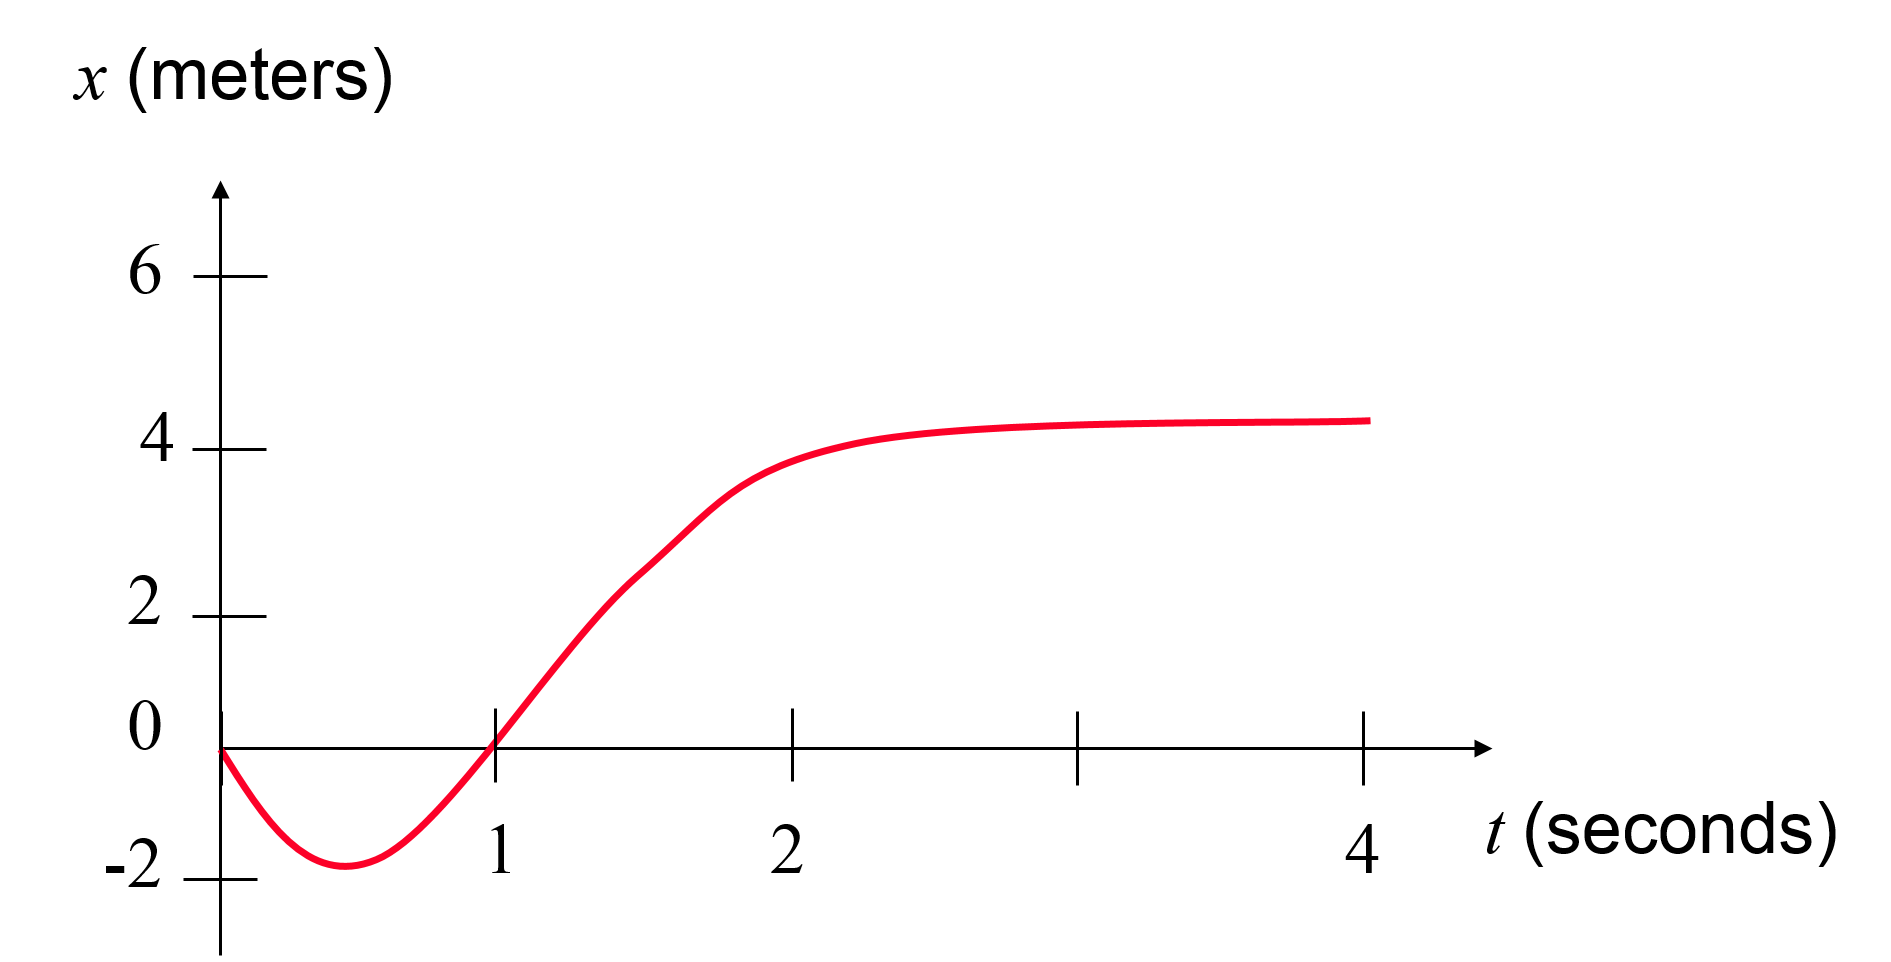
\includegraphics[width=\linewidth]{dfig1.png}
		}
\end{columns}
\end{frame}
\end{iclicker}

%%%%%%%%%%%%%%%%%%%%%%%%%%%%%%%%%
\begin{frame}{Calculus: Derivatives}
Given $f(x)$,\\
\flb \frac{df}{dx} &= \lim_{\epsilon\to 0} \frac{f(x+\epsilon)-f(x)}{\epsilon}& \fle
\flb f(x) &= x^n\quad\qquad\ \  \frac{df}{dx} = n x^{n-1}&\\
	f(x) &= \sin(x)\qquad   \frac{df}{dx} = \cos x&\\
	f(x)&= \cos(x)\qquad  \frac{df}{dx} = -\sin x&
\fle
\end{frame}

%%%%%%%%%%%%%%%%%%%%%%%%%%%%%%%%%
\begin{frame}{Calculus: Integrals}
\begin{columns}
	\column{0.5\linewidth}
		Definite: \flb &\int_a^b f(x)\ dx& \fle
		\flb \int_a^b x^n\ dx&= \frac{x^{n+1}}{n+1}\bigg|^a_b&\\
			&= \frac{a^{n+1}}{(n+1)}-\frac{b^{n+1}}{(n+1)}&\fle
	\column{0.5\linewidth}
		\vspace{-10mm}\\
		Indefinite: \flb &\int f(x)\ dx&\fle 
		\flb \int x^n\ dx &= \frac{x^{n+1}}{(n+1)}+C&\fle 
\end{columns}
\end{frame}


%%%%%%%%%%%%%%%%%%%%%%%%%%%%%%%%%
\begin{frame}{1D Kinematic Equations: Derivation}
\begin{itemize}
	\item Fundamental Theorem of Calculus
	\item $\vect a = \text{constant}$
	\item Boundaries
\end{itemize}
\end{frame}

%%%%%%%%%%%%%%%%%%%%%%%%%%%%%%%%%
\begin{frame}{1D Kinematic Equations}
	\begin{columns}
		\column{0.5\linewidth}
		\vspace{-32mm}\\
		\visible<1->{
			Arbitrary Time Interval:
			\\ 
			\flb v(t_f) - v(t_i) &= a(t_f - t_i)&\fle
			\flb x(t_f)-x(t_i) &= v(t_i) + \frac12 a(t_f-t_i)^2&\fle
		}
		\column{0.5\linewidth}
		\vspace{4mm}\\
		\visible<2->{
			Initial Time Interval:
			\\ \vspace{3mm}
			$t_i=0$,\quad $t_f = t$\\ $v(0) = v_0$,\quad $x(0)=x_0$
			\\ \vspace{1mm}
			\flb \Aboxed{v(t) &= v_0 + a t}&\fle
			\flb \Aboxed{x(t) &= x_0 + v_0t + \frac12 at^2} &\fle
			\\
		}
		\visible<3->{ Solve for common $t$:
				\\ \vspace{-3mm}
				\flb \Aboxed{2a(x-x_0) &= v^2 - v_0^2}&\fle
				}
	\end{columns}
\end{frame}

%%%%%%%%%%%%%%%%%%%%%%%%%%%%%%%%%
\begin{myproblem}
\begin{frame}{Example: Velocity Integration}
	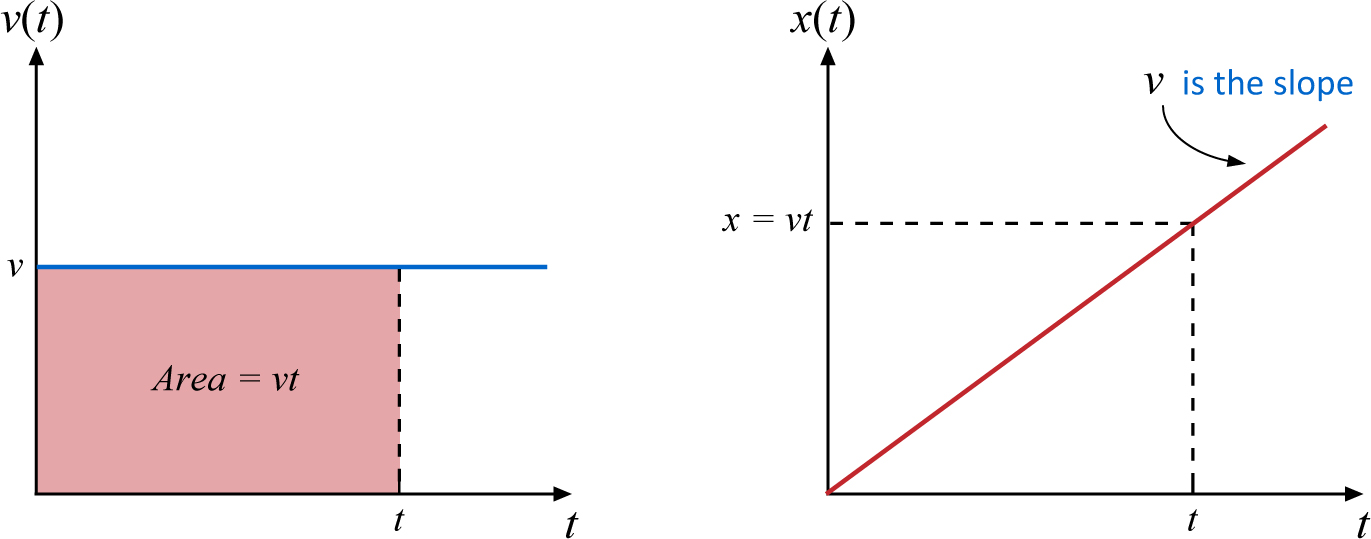
\includegraphics[width=\linewidth]{fig4.jpg}
	\\
	\flb \int_a^b v(t)\ dt &= \int_a^b \left(\frac{dx}{dt}\right)\ dt&\\
		&= x(b) - x(a)& \fle
\end{frame}
\end{myproblem}

%%%%%%%%%%%%%%%%%%%%%%%%%%%%%%%%%
\begin{iclicker}
\begin{frame}{iClicker 4}
The position of a particle is given by
\[	x(t) = 6t - 3t^2.\]
Determine the $x$ position at which the particle's velocity is zero.
\begin{columns}
	\column{0.4\linewidth}
		\begin{enumerate}
			\only<1>{\item $\unit[3]{m}$}
			\only<2>{%
					\item \tikzmark{bl}$\unit[3]{m}$\tikzmark{br}
					\tikz[overlay,remember picture]{\draw[red,thick]
	  				($(bl)+(-2.2em,1.0em)$) rectangle
	 				 ($(br)+(0.3em,-0.4em)$);}}
			\item $\unit[2]{m}$
			\item $\unit[-1]{m}$
			\item $\unit[-3]{m}$
		\end{enumerate}
		\column{0.6\linewidth}
		\visible<2->{
			\flb v&= \frac{dx}{dt} = 6-6t&\fle
			\vspace{-5mm}
			\flb 6-6t &=0&\fle
			\vspace{-5mm}
			\flb t &= 1&\fle
			\vspace{-5mm}
			\flb x(1)&= \unit[3]{m}&\fle}
\end{columns}
\end{frame}
\end{iclicker}

%%%%%%%%%%%%%%%%%%%%%%%%%%%%%%%%%
\begin{iclicker}
\begin{frame}{iClicker 5}
At which point is the speed the greatest?
\begin{columns}
	\column{0.2\linewidth}
		\begin{enumerate}
			\item P
			\item Q
			\only<1>{\item R}
			\only<2>{%
					\item \tikzmark{bl}R\tikzmark{br}
					\tikz[overlay,remember picture]{\draw[red,thick]
	  				($(bl)+(-2.2em,1.0em)$) rectangle
	 				 ($(br)+(0.3em,-0.4em)$);}}
			\item S
		\end{enumerate}
	\column{0.8\linewidth}
	\resizebox{1\linewidth}{!}{
		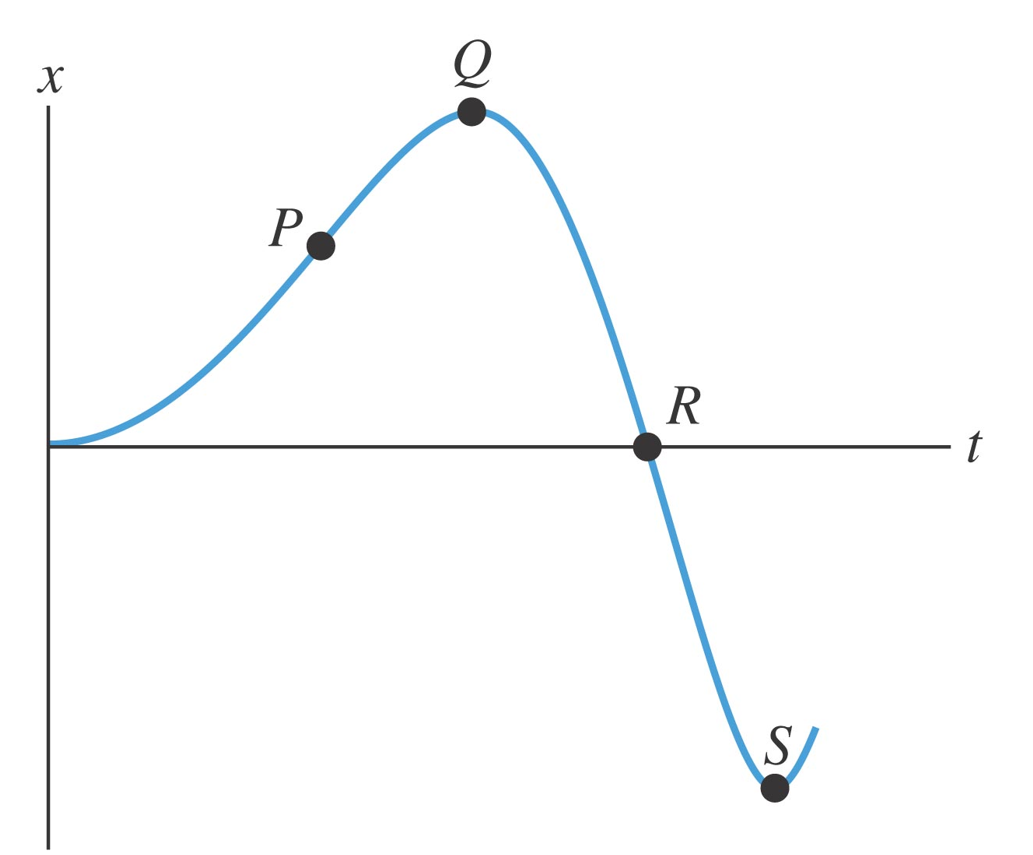
\includegraphics[width=\linewidth]{bfig1.png}
		}
\end{columns}
\end{frame}
\end{iclicker}

%%%%%%%%%%%%%%%%%%%%%%%%%%%%%%%%%
\begin{iclicker}
\begin{frame}{iClicker 6}
At which point does the object have maximum positive velocity?
\begin{columns}
	\column{0.2\linewidth}
		\begin{enumerate}
			\only<1>{\item P}
			\only<2>{%
					\item \tikzmark{bl}P\tikzmark{br}
					\tikz[overlay,remember picture]{\draw[red,thick]
	  				($(bl)+(-2.2em,1.0em)$) rectangle
	 				 ($(br)+(0.3em,-0.4em)$);}}
			\item Q
			\item R
			\item S
		\end{enumerate}
	\column{0.8\linewidth}
	\resizebox{1\linewidth}{!}{
		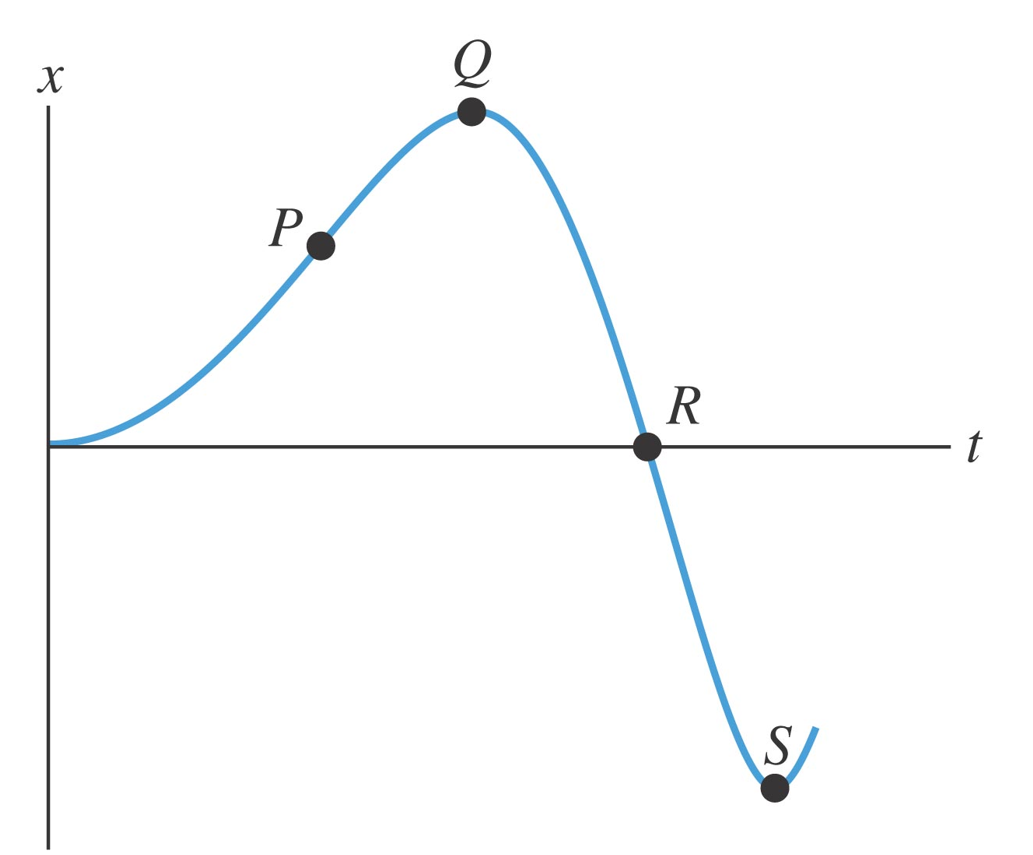
\includegraphics[width=\linewidth]{bfig1.png}
		}
\end{columns}
\end{frame}
\end{iclicker}

%%%%%%%%%%%%%%%%%%%%%%%%%%%%%%%%%
\begin{myproblem}
\begin{frame}{Example: Vertical Ball Throw}
A ball is thrown upward vertically from an initial height of $\unit[5]{m}$ and with an initial velocity of $\unit[10]{m/s}$. Determine $x(t)$, $v(t)$, and the maximum height the ball reaches. \\ \vspace{5mm}
What time does it hit the ground?
\end{frame}
\end{myproblem}

%%%%%%%%%%%%%%%%%%%%%%%%%%%%%%%%%%
%\begin{myproblem}
%\begin{frame}{Example: Two Stage Rocket}
%%Problem set cumulative 18
%A two-stage rocket blasts off vertically from rest on a launch pad. During the first stage, which lasts for \unit[15]{s}, the acceleration is a constant \unit[2]{m/s} upward. At the end of the first stage the second stage engine fires, producing an upward acceleration of \unit[3]{m/s} that lasts for \unit[10]{s}. At the end of the second stage, the engines no longer fire and therefore cause no acceleration, so the rocket coasts to its maximum altitude. Over the time interval from blastoff at the launch pad to the instant that the rocket falls back to the launch pad, ignore the effects of air resistance. 
%\\ \vspace{5mm}
%What is the maximum altitude of the rocket? 
%\\ \vspace{5mm}
%What is its average speed?
%\\ \vspace{5mm}
%What is its average velocity?
%\end{frame}
%\end{myproblem}

%%%%%%%%%%%%%%%%%%%%%%%%%%%%%%%%%
\begin{frame}{Reminders}
\begin{itemize}
	\item 1D Kinematics Homework due Tuesday Sep. 4 (11:59PM)
	\item Vectors and 2D Kinematics Prelecture and Checkpoint due Wednesday Sep. 5 (11:25 AM)
	\item Lab begins week of Sep. 10 
	\begin{itemize}
		\item Lab Notebook
		\item Safety Glasses
		\item Ruler/Calculator
	\end{itemize}
\end{itemize}
\end{frame}


\end{document}